\documentclass[12pt, titlepage]{article}

\usepackage{booktabs}
\usepackage{tabularx}
\usepackage{hyperref}
\hypersetup{
    colorlinks,
    citecolor=black,
    filecolor=cyan,
    linkcolor=red,
    urlcolor=blue
}
\usepackage[round]{natbib}
\usepackage{graphicx}
\graphicspath{ {img/} }

\title{SE 3XA3: Test Plan\\ReTouch}

\author{Team \#7, ReTouchers
		\\ Abrar Attia - attiaa1
		\\ Susan Fayez - fayezs
		\\ Mediha Munim - munimm
}

\date{\today}

\begin{document}

\maketitle

\pagenumbering{roman}
\tableofcontents
\listoftables
\listoffigures

\begin{table}[bp]
\caption{\bf Revision History}
\begin{tabularx}{\textwidth}{p{3cm}p{2cm}X}
\toprule {\bf Date} & {\bf Version} & {\bf Notes}\\
\midrule
October 27 & 1.0 & PoC, and Unit Tests added\\
October 27 & 1.1 & Added general information\\
October 27 & 1.2 & Added System Test Description\\
\bottomrule
\end{tabularx}
\end{table}

\newpage

\pagenumbering{arabic}

This document describes the test plan that shall be followed for ReTouch.

\section{General Information}

\subsection{Purpose}

	The purpose of this project is to re-implement the open source project K-Touch. K-Touch is a utility that allows users to track their speed and accuracy in typing, and results in improved typing skills through practice and repetition. The re-implementation will improve upon the original project by making it more user friendly and providing more comprehensive documentation. The purpose of this document is to make the testing for ReTouch as efficient as possible to ensure a robust, complete, and fully-functional program.

\subsection{Scope}

	The scope of ReTouch will be to improve KTouch by making it available on other operating systems while improving much of the functionality and user experience, while still providing an intuitive GUI and a user guide. Therefore, testing ReTouch will involve testing the GUI, the user input, file input and output, and the other algorithms. 

\subsection{Acronyms, Abbreviations, and Symbols}
	
\begin{table}[hbp]
\caption{\textbf{Table of Abbreviations}} \label{Table}

\begin{tabularx}{\textwidth}{p{3cm}X}
\toprule
\textbf{Abbreviation} & \textbf{Definition} \\
\midrule
GUI & Graphical User Interface\\
Abbreviation2 & Definition2\\
\bottomrule
\end{tabularx}

\end{table}

\begin{table}[!htbp]
\caption{\textbf{Table of Definitions}} \label{Table}

\begin{tabularx}{\textwidth}{p{3cm}X}
\toprule
\textbf{Term} & \textbf{Definition}\\
\midrule
Term1 & Definition1\\
Term2 & Definition2\\
\bottomrule
\end{tabularx}

\end{table}	

\subsection{Overview of Document}

	This document outlines several types of tests that the ReTouchers team plans to use, potential testing tools, a testing schedule, and specific test cases that will cover the functional and non-functional requirements of ReTouch. 

\section{Plan}
	
\subsection{Software Description}

\begin{figure}[h!]
	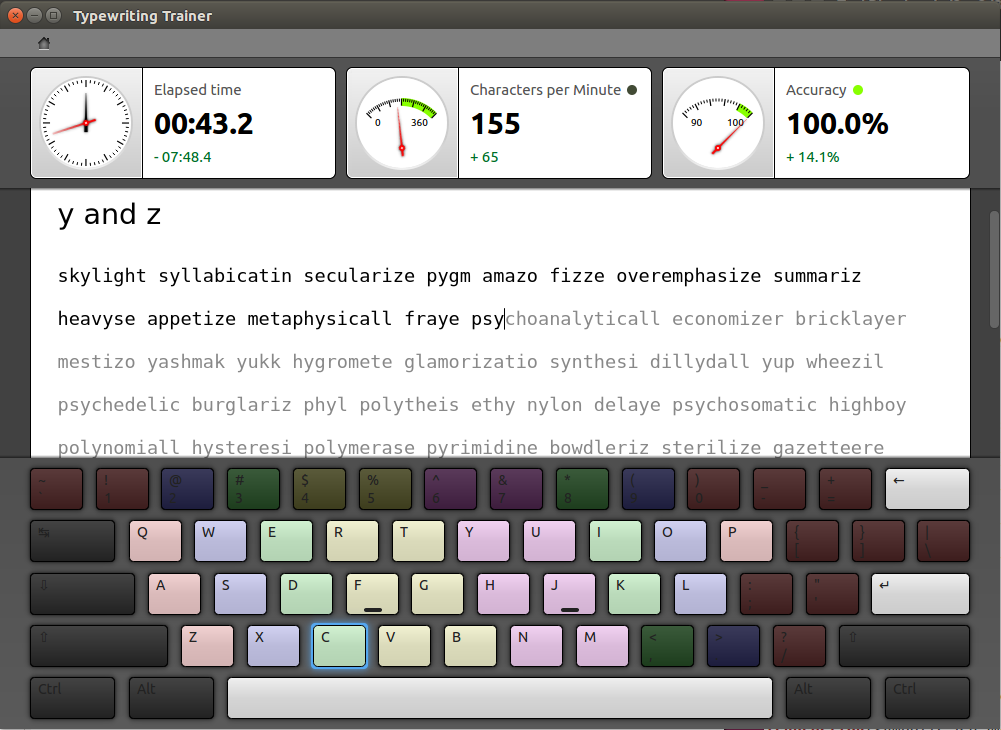
\includegraphics[scale=0.5]{KTouchLesson.png}
	\centering
	\caption{Visual Sample of K-Touch}
	\label{figure:1}
\end{figure}

	ReTouch will be implemented very similarly to K-Touch, the original application, in its functionality. The software shall begin by giving the user a list of lessons to choose from, where each lesson consists of a different combination of keyboard characters that the user can practice typing. The main program will begin at that point. A sequence of characters will appear on screen, and the user will be prompted to type those characters on the keyboard (as is seen in \hyperref[figure:1]{Figure 1}). The user must accurately type all of them (incorrectly typed characters can be erased and then typed again). The software will calculate the elapsed time, the user's typing accuracy, and the user's typing speed during the program's execution. Once the user has completed the lesson, the results of the lesson will appear on screen. The software will be implemented using Java.

\subsection{Test Team}

	The testing will be divided roughly equally among the ReTouchers team (Abrar Attia, Susan Fayez and Mediha Munim). Ideally, every member will be able to look over all of the components that need to be tested and contribute new cases to ensure robustness of the software, but this may not be possible due to the time constraints on the project. See the \hyperref[sec:ts]{Testing Schedule} for details.

\subsection{Testing Approach}

	Many different testing techniques will be utlized in the testing process. Black box testing will involve unit testing and integration testing. To automate these tests, the team will take advantage of JUnit's functionalities. Private methods will be tested as well, and ideally testing will take place throughout the implementation process to ensure that the tests that passed early on in the process will still pass after finalizing the code (regression testing). To test the internal framework of the software, white box testing will be used. Not all of the testing will be automatic - manual system testing will be vital to the final product because the project is expected to have a detailed GUI. Both static and dynamic test cases will be covered using tools described in \hyperref[sec:tt]{Testing Tools}. In system testing, the functionalities of KTouch can be compared to ReTouch to ensure that it works just as it was intended to by the original programmers. All in all, the ReTouchers team strives to test as efficiently and effectively as possible.

\subsection{Testing Tools}
\label{sec:tt}

	As mentioned earlier, the main tool for testing the Java code will be JUnit. Static testing can take place automatically as the project will be implemented in Eclipse, which has static testing capabilities. JaCoCo is a code coverage tool that works well with Eclipse. However, due to the time constraints associated with the project and the potential learning curve with the library, it may not be used. Finally, Apache JMeter will be used for load testing.

\subsection{Testing Schedule}
\label{sec:ts}
		
The Gantt Project, which illustrates the project schedule, can be found \href{run:../../ProjectSchedule/Gantt_Project.gan}{here} or in the ProjectSchedule directory. 

\section{System Test Description}
	
\subsection{Tests for Functional Requirements}

\subsubsection{User Input}
		
\paragraph{Lesson Selection}

\begin{enumerate}

\item{FREQ1\\}

Type: Functional, Dynamic, Manual.
					
Initial State: Lesson selection (start) screen.
					
Input: The desired Lesson.
					
Output: User redirected to beginning of Lesson screen.
					
How test will be performed: The function that runs the selected Lesson will be run. We will check that the correct Lesson was opened.

\end{enumerate}
\paragraph{Lesson Execution}
\begin{enumerate}
    					
\item{FREQ4\\}

Type: Functional, Dynamic, Manual.
					
Initial State: Beginning of the Lesson screen.
					
Input: A desired Lesson.
					
Output: The Lesson is run, the system sets the current character to the first character in the Lesson.
					
How test will be performed: The function that runs the selected Lesson will be run. We will check that the current character value is set to the first character in the given Lesson.

					
\item{FREQ5\\}

Type: Functional, Dynamic, Manual.
					
Initial State: During a Lesson.
					
Input: User types any character.
					
Output: The system moves the current character value to the next one in the Lesson.
					
How test will be performed: The function that runs the Lesson will be run, user input will be provided. We will check the current character value for each time a character is entered to make sure it is being updated properly.

					
\item{FREQ6\\}

Type: Functional, Dynamic, Manual.
					
Initial State: During a Lesson
					
Input: User types the correct current character in the Lesson.
					
Output: The system sets that particular character in the Lesson as completed correctly.
					
How test will be performed: The function that runs the Lesson will be run and user input will be entered. We will check that the system only marked the characters entered correctly will be marked as such.

\item{FREQ8\\}

Type: Functional, Dynamic, Manual.
					
Initial State: During the Lesson, when the user reaches the end of a line.
					
Input: The user hits the enter key.
					
Output: If the user has completed the entire line correctly, they can move on to the next line. If not, they are informed that they must go back and fix their mistakes.
					
How test will be performed: The function that runs the Lesson will be run and user input for the first line will be entered. When the enter button is pressed, we will check if the system gives the proper response, either allowing the user to continue on to the next line, or prompt them to fix their mistakes, depending on whether the input for the line was correct or not.

\item{FREQ14\\}

Type: Functional, Dynamic, Manual.
					
Initial State: During the Lesson, when the user has finished typing everything.
					
Input: The user hits the enter key.
					
Output: If the user has completed the entire Lesson correctly, the Lesson is completed.
					
How test will be performed: The function that runs the Lesson will be run and the user input will be entered for the entire Lesson. We will check to make sure the system terminates the Lesson after the correct input is entered for the entire Lesson and the enter key is entered.

\end{enumerate}

\paragraph{Lesson Mistakes and Corrections}

\begin{enumerate}

\item{FREQ7\\}

Type: Functional, Dynamic, Manual.
					
Initial State: During the Lesson.
					
Input: The user enters an incorrect character.
					
Output: The system highlights the the character that was entered incorrectly, and if the user continues typing, each character after the initial incorrect character is highlighted as incorrect.
					
How test will be performed: The function that runs the Lesson will be run and the user input will be entered incorrectly. We will check that the appropriate characters will be highlighted as incorrect.

\item{FREQ9\\}

Type: Functional, Dynamic, Manual.
					
Initial State: During the Lesson.
					
Input: The user enters he backspace key.
					
Output: The current character is moved to the previous character in the Lesson. If the current character is the first in the Lesson and backspace is entered, nothing happens.
					
How test will be performed: The function that runs the Lesson will be run and user input will be entered. The backspace key will be entered and we will check that the current character has moved appropriately.

\item{FREQ10\\}

Type: Functional, Dynamic, Manual.
					
Initial State: During the Lesson.
					
Input: User input for the Lesson, with some mistakes.
					
Output: The number of characters entered incorrectly is stored in a variable.
					
How test will be performed: The function that runs the Lesson will be run and user input will be entered, with several mistakes. We will check that the counter variable for the number of mistakes is equal to the actual number of mistakes.
\end{enumerate}

\subsubsection{Display}
\paragraph{Lesson Generation}

\begin{enumerate}

\item{FREQ2\\}

Type: Functional, Dynamic, Manual.
					
Initial State: Lesson selection screen
					
Input: The user selects a Lesson
					
Output: The system will generate a Lesson, a list of characters, of less than MAX\_LESSON characters, including spaces.
					
How test will be performed: The function that runs the Lesson will be run and we will check that the Lesson generated is appropriate. 

\end{enumerate}

\paragraph{Lesson Display}

\begin{enumerate}


\item{FREQ3\\}

Type: Structural
					
Initial State: The beginning of the Lesson.
					
Input: The user works on the Lesson.
					
Output: The system displays the list of characters in the Lesson. The list of characters will be presented on separate lines, with each line being no greater than constant MAX\_LINE.

					
How test will be performed: The function that runs the Lesson will be run and we will check that the Lesson is displayed.

\item{FREQ11\\}

Type: Structural
					
Initial State: During the Lesson.
					
Input: The user works on the Lesson.
					
Output: The system displays the elapsed time, from when the user began the Lesson.
					
How test will be performed:  The function that runs the Lesson will be run and we will check that the timer is displayed.

\item{FREQ12\\}

Type: Structural
					
Initial State: During the Lesson.
					
Input: The user works on the Lesson.
					
Output: The system displays the user's typing accuracy.
					
How test will be performed:  The function that runs the Lesson will be run and we will check that the user accuracy is displayed correctly. 

\item{FREQ13\\}

Type: Structural
					
Initial State: During the Lesson
					
Input: The user works on the Lesson
					
Output: The system displays the user's typing speed
					
How test will be performed:  The function that runs the Lesson will be run and we will check that the user's typing speed is displayed correctly.  

\item{FREQ15\\}

Type: Structural
					
Initial State: The Lesson is completed
					
Input: The user hits enter after they finish the Lesson
					
Output: The results (time, typing accuracy, and typing speed) are displayed to the user.
		
How test will be performed: The function that runs the Lesson will be run and the user input will be entered correctly. When the user has completed the Lesson, we will check that the results are properly displayed.

\end{enumerate}
...

\subsection{Tests for Nonfunctional Requirements}

\subsubsection{Look and Feel}

\begin{enumerate}

\item{NFREQ4}

Type: Structural, Static, Manual
					
Initial State: Any screen of the application (Lesson Selection, Lesson, Results).
					
Input/Condition: The user navigates the application.
					
Output/Result: The GUI’s components will be consistent in colour,text  fonts,  and  window  properties  in  order  to  keep the application organized and easy to navigate
					
How test will be performed: We will navigate all three stages of the application to ensure that the aesthetic is consistent throughout.

\end{enumerate}

\subsubsection{Usability and Humanity}
\begin{enumerate}

\item{NFREQ5\\}

Type: Structural, Static, Manual
					
Initial State: The Lesson selected and about to begin.
					
Input/Condition: The user asked to complete the lesson, with no further guidance.
					
Output/Result: The user should be able to complete the lesson.
					
How test will be performed: A test group of users unfamiliar with the application will be asked to test it out.

\item{NFREQ6\\}

Type: Structural, Static, Manual
					
Initial State: The application unopened.
					
Input/Condition: The user asked to complete the process of opening the application, selecting a Lesson, and viewing the results, without further guidance.
					
Output/Result: The user should be able to easily navigate the three stages of the application.
					
How test will be performed:  A test group of users unfamiliar with the application will be asked to test it out.

\item{NFREQ7\\}

Type: Structural, Static, Manual
					
Initial State: The application opened, the Lesson unselected.
					
Input/Condition: User asked to try various Lessons of varying difficulty.
					
Output/Result: The user should find at least one Lesson challenging/helpful in improving their typing skills.
					
How test will be performed:  A test group of users unfamiliar with the application, of varying levels of typing proficiency will be asked to test it out.

\item{NFREQ8\\}

Type: Structural, Static, Manual
					
Initial State: The application not yet installed.
					
Input/Condition: The user asked to install the application.
					
Output/Result: The application should be easy for for the user to install.
					
How test will be performed:  A test group of users unfamiliar with the application will be asked to install the application.

\end{enumerate}
\subsubsection{Performance}
\begin{enumerate}

\item{NFREQ9\\}

Type: Structural, Dynamic, Manual
					
Initial State: During the Lesson.
					
Input/Condition: The user works on the Lesson.
					
Output/Result: The system will respond to the user input within 1 second.
					
How test will be performed: A user will work through a Lesson and we will check the response time as they go. 

\item{NFREQ10\\}

Type: Structural, Dynamic, Manual
					
Initial State: During the Lesson.
					
Input/Condition: The user works on the Lesson.
					
Output/Result: The timer displayed to the user will be accurate and begin once the user enters their first character, and will end once the user hits enter to complete the Lesson.
					
How test will be performed: A user will work on a Lesson and we will check that the timer is accurate.

\item{NFREQ13\\}

Type: Structural, Static, Manual
					
Initial State: Any point in using the application.
					
Input/Condition: The user uses the application.
					
Output/Result: The application will not interfere with the user's machine.
					
How test will be performed: We will check on the user's machine during and after the application runs, to ensure everything is running properly.

\end{enumerate}
\subsubsection{Operation and Environment}
\begin{enumerate}

\item{NFREQ14\\}

Type: Structural, Static, Manual
					
Initial State: Application installed on a Windows and a Linux machine.
					
Input/Condition: User runs the application on both machines.
					
Output/Result: The application should run smoothly on both machines.
					
How test will be performed: Run the application on both machines.

\item{NFREQ15\\}

Type: Structural, Static, Manual
					
Initial State: The application is unopened.
					
Input/Condition: The user opens the application.
					
Output/Result: The application depends on no other applications to run properly.
					
How test will be performed: We will open the application independently of any other applications.

\end{enumerate}

\subsubsection{Security}
\begin{enumerate}

\item{NFREQ17\\}

Type: Structural, Static, Manual
					
Initial State: During a Lesson.
					
Input/Condition: The user completes the Lesson.
					
Output/Result: The system will not store any information on the user's results. 
					
How test will be performed: When the user completes their lesson, we will check to make sure none of the data is stored.

\end{enumerate}
\subsubsection{Cultural}
\begin{enumerate}

\item{NFREQ19\\}

Type: Structural, Static, Manual
					
Initial State: The application is unopened.
					
Input/Condition: A user will be asked to open and go through the three stages of the application (Lesson Selection, Lesson, and Results).
					
Output/Result: The user shall not be offended by any of the content within the application.
					
How test will be performed: A test group of users unfamiliar with the application will be asked to use the application. 
\end{enumerate}

\section{Tests for Proof of Concept}

The Proof of Concept testing will focus on validating that all the identified risks in the development of the application can be overcome. The determined risks that can be tested focuses on running the code concurrently. The current program implements a constant timer alongside a main program that requests and waits for keyboard input. 

\subsection{Running Programs Concurrently}
		
\paragraph{Constant Timer and User Input Verification}

\begin{enumerate}

\item{FC-1\\}

Type: Functional, Dynamic, Manual
					
Initial State: no input is set
					
Input: User inputs characters
					
Output: Calculated accuracy of user to match the expected characters
					
How test will be performed: The user will be requested to input a certain character as the timer waits for their input. The final characters inputted will be compared to the initial requested characters to determine the users accuracy.Therefore, half the program that tests the users keyboard inputs will be tested. 
					
\item{FC-2\\}

Type: Functional, Dynamic, Manual
					
Initial State: no input is set
					
Input: User inputs characters
					
Output: The total time taken in comparison to the expected time, and the users speed calculation; the total characters per second.
					
How test will be performed: As the user inputs characters that are requested, the timer will be tracked. Once the lesson is run through, the total time the program records will be compared to the expected time. Also, the users speed calculation will be compared to the expected characters per second to confirm that the timer is running efficiently. Therefore, such test will confirm that the two programs are running concurrently and both sections are being completed successfully.

\end{enumerate}

	
\section{Comparison to Existing Implementation}	
There is currently no required tests to be done to compare the application to the existing implementation.
				
\section{Unit Testing Plan}

The JUnit unit testing framework will be used to implement the unit testing for the ReTouch application.
		
\subsection{Unit testing of internal functions}

When testing the internal functions of the application, the unit tests will be based on each methods input parameters and their expected versus derived outputs. Each method will be testing with standard expected inputs as well as exceptions to improve the programs robustness and reduce bugs. Additionally, every class in the program will include all the required import statements. Therefore, the unit tests will not require any stubs or drivers when testing individual methods or components that depend on multiple methods. In addition, coverage metrics will be used to determine how much of the implemented code was tested. The goal percentage to reach is 80\%. 
		
\subsection{Unit testing of output files}

When testing the output files and program outputs, there will need to be a comparison between the required output and the generated output. However, at this time, there are no expected output files that will be created when the program is run. 		

\bibliographystyle{plainnat}

\bibliography{SRS}

\newpage

\subsection{Symbolic Parameters}

The definition of the test cases will call for SYMBOLIC\_CONSTANTS.
Their values are defined in this section for easy maintenance.

\subsection{Usability Survey Questions?}

This is a section that would be appropriate for some teams.

\end{document}
